\documentclass{standalone}
\usepackage{tikz}

\begin{document}

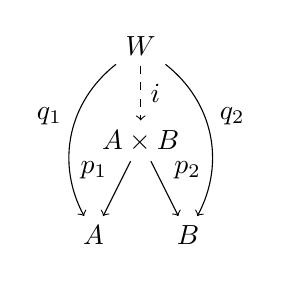
\begin{tikzpicture}[auto]
    \node (W) at (0.6, 2.4) {$W$};
    \node (T) at (0.6, 1.2) {$A \times B$};
    \node (A) at (0, 0) {$A$}; \node (B) at (1.2, 0) {$B$};
    \draw[->] (T) to node[swap] {$p_1$} (A);
    \draw[->] (T) to node {$p_2$} (B);
    \draw[->] (W) to[bend right=40] node[swap] {$q_1$} (A);
    \draw[->] (W) to[bend left=40] node {$q_2$} (B);

    \draw[->, dashed] (W) to node {$i$} (T);
    
\end{tikzpicture}

\end{document}
